%%%%%%%%%%%%%%%%%%%%%%%%%%%%%%%%%%%%%%%%%
% Masters/Doctoral Thesis 
% LaTeX Template
% Version 2.5 (27/8/17)
%
% This template was downloaded from:
% http://www.LaTeXTemplates.com
%
% Version 2.x major modifications by:
% Vel (vel@latextemplates.com)
%
% This template is based on a template by:
% Steve Gunn (http://users.ecs.soton.ac.uk/srg/softwaretools/document/templates/)
% Sunil Patel (http://www.sunilpatel.co.uk/thesis-template/)
%
% Template license:
% CC BY-NC-SA 3.0 (http://creativecommons.org/licenses/by-nc-sa/3.0/)
%
% // ========= //
%
% This template has been partially modified by Alejandro Rodríguez López
%
%%%%%%%%%%%%%%%%%%%%%%%%%%%%%%%%%%%%%%%%%

%----------------------------------------------------------------------------------------
%	PACKAGES AND OTHER DOCUMENT CONFIGURATIONS
%----------------------------------------------------------------------------------------

\documentclass[
11pt, % The default document font size, options: 10pt, 11pt, 12pt
oneside, % Two side (alternating margins) for binding by default, uncomment to switch to one side
spanish, % TODO: Set language [english, spanish, ngerman]
singlespacing, % Single line spacing, alternatives: onehalfspacing or doublespacing
%draft, % Uncomment to enable draft mode (no pictures, no links, overfull hboxes indicated)
%nolistspacing, % If the document is onehalfspacing or doublespacing, uncomment this to set spacing in lists to single
%liststotoc, % Uncomment to add the list of figures/tables/etc to the table of contents
%toctotoc, % Uncomment to add the main table of contents to the table of contents
%parskip, % Uncomment to add space between paragraphs
%nohyperref, % Uncomment to not load the hyperref package
headsepline, % Uncomment to get a line under the header
%chapterinoneline, % Uncomment to place the chapter title next to the number on one line
%consistentlayout, % Uncomment to change the layout of the declaration, abstract and acknowledgements pages to match the default layout
]{MastersDoctoralThesis} % The class file specifying the document structure

\usepackage[utf8]{inputenc} % Required for inputting international characters
\usepackage[T1]{fontenc} % Output font encoding for international characters
\usepackage{pgffor}
\usepackage{listings}
\usepackage{hyperref}
\usepackage{xcolor}
\usepackage{tabularx}
\usepackage{listings-rust}
\usepackage{tabularx, multirow}
\usepackage{amsmath}

\colorlet{punct}{red!60!black}
\definecolor{background}{HTML}{EEEEEE}
\definecolor{delim}{RGB}{20,105,176}
\colorlet{numb}{magenta!60!black}

\lstdefinelanguage{json}{
    basicstyle=\normalfont\ttfamily,
    numbers=left,
    numberstyle=\scriptsize,
    stepnumber=1,
    numbersep=8pt,
    showstringspaces=false,
    breaklines=true,
    frame=lines,
    backgroundcolor=\color{background},
    literate=
     *{0}{{{\color{numb}0}}}{1}
      {1}{{{\color{numb}1}}}{1}
      {2}{{{\color{numb}2}}}{1}
      {3}{{{\color{numb}3}}}{1}
      {4}{{{\color{numb}4}}}{1}
      {5}{{{\color{numb}5}}}{1}
      {6}{{{\color{numb}6}}}{1}
      {7}{{{\color{numb}7}}}{1}
      {8}{{{\color{numb}8}}}{1}
}

\definecolor{lightgray}{rgb}{.9,.9,.9}
\definecolor{darkgray}{rgb}{.4,.4,.4}
\definecolor{purple}{rgb}{0.65, 0.12, 0.82}

\lstdefinelanguage{JavaScript}{
  keywords={const, let, var, typeof, new, true, false, catch, function, return, null, catch, switch, var, if, in, while, do, else, case, break},
  keywordstyle=\color{blue}\bfseries,
  ndkeywords={class, export, boolean, throw, implements, import, this},
  ndkeywordstyle=\color{darkgray}\bfseries,
  identifierstyle=\color{black},
  sensitive=false,
  comment=[l]{//},
  morecomment=[s]{/*}{*/},
  commentstyle=\color{purple}\ttfamily,
  stringstyle=\color{red}\ttfamily,
  morestring=[b]',
  morestring=[b]"
}

\lstset{
   backgroundcolor=\color{lightgray},
   extendedchars=true,
   basicstyle=\footnotesize\ttfamily,
   showstringspaces=false,
   showspaces=false,
   numbers=left,
   numberstyle=\footnotesize,
   numbersep=9pt,
   tabsize=2,
   breaklines=true,
   showtabs=false,
   captionpos=b
}

\usepackage{enumitem}
\usepackage{tikz-uml}
% Remove the problematic code
\usepackage{float}

\usepackage{tcolorbox}
\newtcolorbox{notebox}{
  colback=white,
  colframe=black,
  boxrule=1pt,
  arc=4pt,
  fonttitle=\bfseries,
  title=NOTA
}

\newtcolorbox{examplebox}{
  colback=white,
  colframe=blue,
  boxrule=1pt,
  arc=4pt,
  fonttitle=\bfseries,
  title=EJEMPLO
}

\usepackage{mathpazo} % Use the Palatino font by default
%\usepackage[backend=bibtex,style=authoryear,natbib=true,language=english]{biblatex} % Use the bibtex backend with the authoryear citation style (which resembles APA)

%\addbibresource{bibliography.bib} % The filename of the bibliography

\usepackage[autostyle=true]{csquotes} % Required to generate language-dependent quotes in the bibliography
\usepackage{titlesec}

\newcommand{\bold}[1]{\textbf{#1}\ }
\newcommand{\italic}[1]{\textit{#1}\ }
\newcommand{\frontend}{\bold{frontend}}
\newcommand{\backend}{\bold{backend}}
\newcommand{\ReactJS}{\href{https://react.dev/}{\bold{ReactJS}}}
\newcommand{\Flask}{\href{https://flask.palletsprojects.com/en/3.0.x/}{\bold{Flask}}}
\newcommand{\SQLAlchemy}{\href{https://www.sqlalchemy.org/}{\bold{SQL Alchemy}}}
\newcommand{\TypeScript}{\href{https://www.typescriptlang.org/}{\bold{TypeScript}}}
\newcommand{\JavaScript}{\href{https://www.javascript.com/}{\bold{JavaScript}}}
\newcommand{\Python}{\href{https://www.python.org/}{\bold{Python}}}
\newcommand{\Java}{\href{https://www.java.com/en/}{\bold{Java}}}
\newcommand{\Rust}{\href{https://www.rust-lang.org/}{\bold{Rust}}}
\newcommand{\C}{\href{https://en.wikipedia.org/wiki/C_(programming_language)}{\bold{C}}}
\newcommand{\Haskell}{\href{https://www.haskell.org/}{\bold{Haskell}}}

\newcommand\Chapter[2]{
  \chapter[#1: {\itshape#2}]{#1\\\hfill\Large\itshape#2}
  \label{chap:#1}
}

\newcommand\Section[1]{\section{#1}\label{sec:#1}}
\newcommand\Subsection[1]{\subsection{#1}\label{ssec:#1}}
\newcommand\Subsubsection[1]{\subsubsection{#1}\label{sssec:#1}}
\newcommand\Paragraph[1]{\paragraph{#1}\label{par:#1}}

\newcommand\uml[2]{
  \begin{figure}[h]
    \begin{center}
      #1
    \end{center}
    \caption{#2}
  \end{figure}
}

%----------------------------------------------------------------------------------------
%	PARAGRAPH SETTINGS
%----------------------------------------------------------------------------------------

\setlength{\parskip}{\baselineskip}%

%----------------------------------------------------------------------------------------
%	MARGIN SETTINGS
%----------------------------------------------------------------------------------------

\geometry{
	paper=a4paper, % Change to letterpaper for US letter
	inner=2.5cm, % Inner margin
	outer=3.8cm, % Outer margin
	bindingoffset=.5cm, % Binding offset
	top=1.5cm, % Top margin
	bottom=1.5cm, % Bottom margin
	%showframe, % Uncomment to show how the type block is set on the page
}

%----------------------------------------------------------------------------------------
%	THESIS INFORMATION
%----------------------------------------------------------------------------------------

% Should you want to have an href alongside the name, state it inside the variable using:
% \href{url}{name}

% TODO: Your thesis title, print it with \ttitle
\thesistitle{Copilot inteligente para consultas LINQ/SQL}
% TODO: Your tutor name, print it with \tutor
\tutor{Moldón Redondo, Daniel} 
% TODO: Your other tutor name, print it with \tutorBis
\tutorBis{Costa Cortez, Nahuel Alejandro} 
% TODO: Your degree name, print it with \degreename
\degree{la asignatura Prácticas de Empresa del grado Ingeniería Informática en Tecnologías de la Información} 
% TODO: Your name, print it with \authorname
\author{Puga Lojo, Francisco Gabriel} 
% TODO: Your peer name, print it with \authornameBis
\authorBis{AutorBis} 
% TODO: Your address, print it with \addressname
\addresses{Address} 

% TODO: Your subject area, print it with \subjectname
\subject{} 
% TODO: Keywords for your thesis, print it with \keywordnames
\keywords{Keywords} 
% TODO: Your university's name and URL, print it with \univname
\university{UNIVERSIDAD DE OVIEDO} 
% TODO: Your department's name and URL, print it with \deptname
\department{Ingeniería Informática en Tecnologías de la Información} 
% TODO: Your research group's name and URL, print it with \groupname
\group{Group} 
% TODO: Your faculty's name and URL, print it with \facname
\faculty{Escuela Politécnica de Ingeniería de Gijón (EPI)} 

\AtBeginDocument{
	\hypersetup{pdftitle=\ttitle} % Set the PDF's title to your title
	\hypersetup{pdfauthor=\authorname} % Set the PDF's author to your name
	\hypersetup{pdfkeywords=\keywordnames} % Set the PDF's keywords to your keywords
}

\begin{document}

\frontmatter % Use roman page numbering style (i, ii, iii, iv...) for the pre-content pages

\pagestyle{plain} % Default to the plain heading style until the thesis style is called for the body content

%----------------------------------------------------------------------------------------
%	TITLE PAGE
%----------------------------------------------------------------------------------------

\begin{titlepage}
\begin{center}

\vspace*{.06\textheight}
{\scshape\LARGE \univname\\\facname\par}\vspace{1.5cm} % University name
\textsc{\Large \subjectname}\\[0.5cm] % Thesis type

\HRule \\[0.4cm] % Horizontal line
{\huge \bfseries \ttitle\par}\vspace{0.4cm} % Thesis title
\HRule \\[1.5cm] % Horizontal line
 
\begin{minipage}[t]{\textwidth}
	\begin{flushleft} \large
		\emph{Autor:}\\
		\authorname\\
    \vspace{2em}
	\end{flushleft}
\end{minipage}
\begin{minipage}[t]{\textwidth}
	\begin{flushleft} \large
    \vspace{2em}
	\end{flushleft}
\end{minipage}
\begin{minipage}[t]{0.8\textwidth}
	\begin{flushright} \large
		\emph{Tutor (Mecalux):} \\
		\tutorName
    \vspace{2em}
	\end{flushright}
\end{minipage}\\
\begin{minipage}[t]{0.8\textwidth}
	\begin{flushright} \large
		\emph{Tutor (EPI):} \\
		\tutorBisName
	\end{flushright}
\end{minipage}\\[3cm]
 
\vfill

% University requirement text
\large\textit{\requirements}\\[0.3cm] 
% \textit{en}\\[0.4cm]
% \groupname\\[2cm] % Research group name and department name
 
\vfill

{\large \today}\\[4cm] % Date
%\includegraphics{Logo} % University/department logo - uncomment to place it
 
\vfill
\end{center}
\end{titlepage}

%----------------------------------------------------------------------------------------
%	DECLARATION PAGE
%----------------------------------------------------------------------------------------

%\begin{declaration}
%\addchaptertocentry{\authorshipname} % Add the declaration to the table of contents
%\noindent Yo, \authorname, declaro que este documento titulado, \enquote{\ttitle} y el trabajo presentado en él son de mi propiedad.
%Afirmo que:

%\begin{itemize} 
	%\item Este trabajo fue realizado completa o parcialmente durante mi estancia como estudiante en el grado de \`degree'name.
	%\item Aquellas partes de este documento que hayan sido previamente publicadas se encuentran debidamente indicadas.
	%\item Aquellas partes de este documento que se apoyen en trabajos previamente publicados se encuentran debidamente indicadas.
	%\item Todas las fuentes utilizadas para la realizacion de este trabajo se encuentran listadas.
%\end{itemize}

%\vfill

%\noindent Signed: \authorname\\
%\rule[0.5em]{25em}{0.5pt} % This prints a line for the signature
 
%\noindent Date: Julio 13, 2023\\
%\rule[0.5em]{25em}{0.5pt} % This prints a line to write the date
%\end{declaration}

%\cleardoublepage

%----------------------------------------------------------------------------------------
%	QUOTATION PAGE
%----------------------------------------------------------------------------------------

%\vspace*{0.2\textheight}

%\noindent\enquote{
	%\itshape Thanks to my solid academic training, today I can write hundreds of words on virtually any topic
	%without possessing a shred of information, which is how I got a good job in journalism.
%}\bigbreak

%\hfill Dave Barry

%----------------------------------------------------------------------------------------
%	ABSTRACT PAGE
%----------------------------------------------------------------------------------------

\begin{abstract}
% TODO: Add the abstract



El manejo de bases de datos es fundamental para la gestión de información en las empresas hoy en día. En un mundo donde la información es clave, poder procesar datos importantes es vital para mantener y hacer crecer una empresa.

Sin embargo, trabajar con bases de datos puede ser complicado y requiere una formación específica que muchas personas fuera del ámbito informatico no tienen ni tiempo para aprender.

Mecalux es una de las compañías líderes en tecnología intralogística a nivel mundial. Es puntera en automatización de almacenes y desarrollo de software. En estas prácticas, he contribuido a desarrollar un asistente que ayuda a generar código \href{https://en.wikipedia.org/wiki/Language_Integrated_Query}{\bold{LINQ}} SQL y que también explica las consultas generadas.

El objetivo de este asistente es facilitar el trabajo de los empleados, permitiéndoles crear y entender consultas SQL sin necesidad de conocimientos técnicos profundos, y simplificando las tareas para quienes sí los tienen. Esto agiliza los procesos internos y mejora la eficiencia en la toma de decisiones, lo cual es crucial en el entorno empresarial actual.
\addchaptertocentry{\abstractname}

\end{abstract}

%----------------------------------------------------------------------------------------
%	ACKNOWLEDGEMENTS
%----------------------------------------------------------------------------------------

%\begin{acknowledgements}
%\addchaptertocentry{\acknowledgementname} % Add the acknowledgements to the table of contents
%The acknowledgments and the people to thank go here, don't forget to include your project advisor\ldots
%\begin{itemize}
	%\item \groupname
		%\begin{itemize}
			%\item \tutorEmpName
			%\item Antiñolo, David Espejo
			%\item Omen, Juan David
			%\item Rico, Luis Rodríguez
		%\end{itemize}
	%\item \facname
		%\begin{itemize}
			%\item \tutorEpiName
		%\end{itemize}
%\end{itemize}
%\end{acknowledgements}

%----------------------------------------------------------------------------------------
%	LIST OF CONTENTS/FIGURES/TABLES PAGES
%----------------------------------------------------------------------------------------

\tableofcontents % Prints the main table of contents

%\listoffigures % Prints the list of figures

%\listoftables % Prints the list of tables

%----------------------------------------------------------------------------------------
%	ABBREVIATIONS
%----------------------------------------------------------------------------------------

\begin{abbreviations}{ll} % Include a list of abbreviations (a table of two columns)

% TODO: Add Abbreviations

\textbf{MSS} & \textbf{M}ecalux \textbf{S}oftware \textbf{S}olutions\\
%\textbf{WSF} & \textbf{W}hat (it) \textbf{S}tands \textbf{F}or\\

\textbf{IT} & \textbf{I}nformation \textbf{T}echnlogies\\
\textbf{I+D+I} & \textbf{I}nvestigación, \textbf{D}esarrollo e \textbf{I}nnovación\\
\textbf{IA} & \textbf{I}nteligencia \textbf{A}rtificial\\
\textbf{LLM} & \textbf{L}arge \textbf{L}anguage \textbf{M}odel\\
\textbf{LoRA} & \textbf{L}ow \textbf{R}ank \textbf{A}daptation\\
\textbf{CUDA} & \textbf{C}ompute \textbf{U}nified \textbf{D}evice \textbf{A}rchitecture\\
\textbf{POO} & \textbf{P}rogramación \textbf{O}rientada a \textbf{O}bjetos\\
\textbf{RAG} & \textbf{R}etrieval \textbf{A}ugmented \textbf{G}eneration\\

%\textbf{E} & Número de \textbf{E}mpleadores\\
%\textbf{I} & \textbf{I}mpuestos calculados a partir de BI\\
%\textbf{P} & Cantidad pagada en \textbf{P}réstamos por hipotecas de vivienda habitual comprada antes de 2013\\
%\textbf{R} & \textbf{R}etenciones\\
%\textbf{SP} & \textbf{S}ituación de \textbf{P}rueba\\

\end{abbreviations}

%----------------------------------------------------------------------------------------
%	PHYSICAL CONSTANTS/OTHER DEFINITIONS
%----------------------------------------------------------------------------------------

%\begin{constants}{lr@{${}={}$}l} % The list of physical constants is a three column table

% The \SI{}{} command is provided by the siunitx package, see its documentation for instructions on how to use it

%Speed of Light & $c_{0}$ & \SI{2.99792458e8}{\meter\per\second} (exact)\\
%Constant Name & $Symbol$ & $Constant Value$ with units\\

%\end{constants}

%----------------------------------------------------------------------------------------
%	SYMBOLS
%----------------------------------------------------------------------------------------

%\begin{symbols}{lll} % Include a list of Symbols (a three column table)

%$a$ & distance & \si{\meter} \\
%$P$ & power & \si{\watt} (\si{\joule\per\second}) \\
%Symbol & Name & Unit \\

%\addlinespace % Gap to separate the Roman symbols from the Greek

%$\omega$ & angular frequency & \si{\radian} \\

%\end{symbols}

%----------------------------------------------------------------------------------------
%	DEDICATION
%----------------------------------------------------------------------------------------

%\dedicatory{For/Dedicated to/To my\ldots} 

%----------------------------------------------------------------------------------------
%	BLANK PAGE
%----------------------------------------------------------------------------------------

%\blankpage

%----------------------------------------------------------------------------------------
%	THESIS CONTENT - CHAPTERS
%----------------------------------------------------------------------------------------

\mainmatter % Begin numeric (1,2,3...) page numbering

\pagestyle{thesis} % Return the page headers back to the "thesis" style
% Include the chapters of the thesis as separate files from the Chapters folder
% Uncomment the lines as you write the chapters

% Chapter 1

\Chapter{Introducción}{El alumno y la empresa}

\href{https://www.mecalux.es/}{\bold{Mecalux}} es una empresa reconocida internacionalmente en el sector de soluciones de almacenamiento. Desde su fundación en 1966, ha desarrollado un amplio portafolio que abarca una variedad de sistemas de almacenamiento, como estanterías, almacenes automatizados y soluciones de software para la gestión de almacenes. 

Con una presencia global, Mecalux opera en numerosos países, gestionando un gran volumen de operaciones y personal especializado. Las prácticas fueron realizadas de manera presencial en las \href{https://maps.app.goo.gl/bJKvSNHAo5t1j4BZ6}{\bold{oficinas de MSS en Gijón.}}\footnote{Mecalux Software Solutions es la división de Mecalux dedicada enteramente al desarrollo de software para almacenes y logística.}

\begin{notebox}
  Aunque las prácticas fueron presenciales, Mecalux tiene una metodología de teletrabajo muy arraigada de la cual muchos empleados de IT siguen beneficiándose. \\ \\
  Es notable cómo esta flexibilidad está bien integrada en su rutina diaria, y parte de la comunicación con el equipo ha sido de de esta manera.
\end{notebox}

Durante estas prácticas de empresa, tuve la oportunidad de formar parte del equipo de Data Analytics en la división de MSS. En el próximo capítulo se detallarán las actividades llevadas a cabo por este equipo, junto con sus metas y objetivos.



% Chapter 1
\Chapter{Data Analytics}{Innovación y solución de problemas}

\section{Contexto}\label{sec:contexto}
He tenido la fortuna de trabajar dentro del departamento de Data Analytics, el cual se encarga de recopilar, limpiar e interpretar conjuntos de datos para responder a preguntas o resolver problemas. Es un equipo muy multidisciplinar, y me sorprendió positivamente que, aunque la mayoría de sus miembros no provienen de estudios de Informática (sino de áreas como Física, Matemáticas, etc.), todos poseen una gran capacidad para reflexionar y resolver problemas de manera lógica, metódica y, sobre todo, en equipo.

Además de su labor como analistas de datos, este equipo también cumple la función de resolver inconvenientes que puedan surgir en otros departamentos y se encarga de investigar y poner a prueba nuevas soluciones antes de su implementación en el entorno de producción. Se podría decir que realizan funciones similares a las de I+D+I, ya que investigan, desarrollan y prueban nuevas soluciones para mejorar los procesos y resolver problemas dentro de la empresa.

Durante mis prácticas, mi labor ha sido una combinación de investigación y desarrollo de software, lo cual ha sido posible gracias a la naturaleza y dinámica de este equipo.


\section{Metodología de Trabajo}
Como se mencionó en la introducción, parte del equipo realiza teletrabajo, algunos de manera ocasional y otros de forma regular. De hecho, hay un integrante que ni siquiera reside en Asturias. El equipo realiza reuniones diarias (dailys), a las cuales tuve el placer de asistir en la última etapa de mis prácticas. En estas reuniones, los miembros explican el progreso y las tareas realizadas el día anterior. Estas reuniones se llevan a cabo en salas especialmente equipadas en el edificio, las cuales cuentan con cámaras y proyectores para que los empleados que están teletrabajando puedan participar activamente en las reuniones.

\subsection{Dinámica de trabajo durante las prácticas}
El departamento estaba enfocado en sus proyectos, por lo que mi equipo de trabajo habitual se 
redujo a otro alumno de prácticas de la carrera de Ingeniería Informática del Software, y nuestro tutor, 
perteneciente a Data Analytics, que se encargaba de que fuésemos por el buen camino y con el que hacíamos
también nuestras propias reuniones diarias para ver el progreso de nuestro trabajo.

Mi compañero y yo teníamos horarios diferentes, por lo que coincidíamos en las oficinas durante un tiempo limitado, lo que conllevó a la necesidad de coordinarnos lo mejor posible y así poder tener los objetivos claros y aprovechar al máximo el tiempo que teníamos juntos para desarrollar, estructurar nuestras tareas y debatir los problemas a los que nos enfrentaríamos. 

Al entrar antes a la oficina, me encargaba de hablar con el tutor para ver si había nuevas opciones que explorar o investigar, por donde seguir si habíamos conseguido los resultados esperados, o en caso contrario comunicar los inconvenientes, y coordinar la planificación para el día. 

De esta manera, cuando mi compañero llegaba, era todo más fácil para los tres, el tutor no necesitaba volver a explicarlo todo y yo podía comunicarle de forma efectiva que teníamos que hacer, las novedades, y como nos podríamos distribuir el trabajo. 

Por otra parte, cuando yo me marchaba mi compañero seguía desarrollando y trabajando en el proyecto, por lo que me comunicaba sus avances por la plataforma de Teams para que cuando llegase al día siguiente supiese de manera más rápida que era lo que se había hecho.

Nuestra comunicación fue en todo momento muy buena, nos sentábamos en mesas próximas por lo que nos acercábamos a hablar sobre como realizar el trabajo frecuentemente, y cuando no queríamos molestar utilizábamos el chat de Teams.

Cabe resaltar que aunque no trabajase con todos los integrantes del departamento de Data Analytics directamente al no pertenecer al proyecto en sí, muchos de ellos me ayudaron  a lo largo de las prácticas y hubo una comunicación cercana y efectiva independientemente de ello.


% Chapter 2
\Chapter{MSSCopilot}{Generación de Código Automática}

\section{Objetivo de las prácticas}
El objetivo principal de las prácticas fue desarrollar una herramienta que permitiera a los usuarios generar código de manera automática. Esta herramienta, denominada MSSCopilot, debía ser capaz de generar código en \href{https://dotnet.microsoft.com/es-es/languages/csharp}{\bold{C\#}} / \href{https://en.wikipedia.org/wiki/Language_Integrated_Query}{\bold{LINQ}} a partir de la base de código fuente existente en la compañía.

\begin{examplebox}

Un empleado le dice al MSSCopilot que desea obtener una lista con todos los Warehouses, el Copilot respondería con un código como el siguiente:

\begin{lstlisting}[language=C]
    using (var context = new MyContext())
    {
        var result = context.Warehouse.Select(x => x);
    }
    \end{lstlisting}
\end{examplebox}        

Durante el desarrollo del programa se elaboraron más funcionalidades de las previstas inicialmente como es la explicación de código, y otras más que se explicarán con mayor profundidad posteriormente.

El estado del proyecto al comenzar las prácticas estaba en una etapa inicial, lo que permitió un entendimiento más profundo del mismo y facilitó la integración de nuevas ideas y funcionalidades desde el principio. 

\section{Desarrollo}

Definir las tecnologías utilizadas en la realización del MSSCopilot resulta complicado porque como se ha comentado en la sección \ref{sec:contexto}, aunque se trate de desarrollar un producto de software, ha sido un proyecto en el que, por la naturaleza de la IA, que sigue siendo un sector de tecnologías emergentes, las directrices a seguir no son tan claras. Debido a esto, gran parte del proyecto ha consistido en un proceso de investigación en el que se han utilizado tecnologías y técnicas que, con el tiempo, se han descartado en favor de otras opciones mejores a medida que se identificaban. Hay mucho trabajo realizado que he omitido porque la memoria de prácticas no pretende ser una memoria técnica, sin embargo, es importante tener en cuenta que estas tecnologías y explicaciones son solo una parte del panorama completo, y el proyecto ha implicado una exploración más amplia de diversas herramientas y enfoques en el campo de la inteligencia artificial.

\subsection{Conocimientos previos}
Los \href{https://en.wikipedia.org/wiki/Large_language_model}{\bold{LLM}} son un tipo de modelo de inteligencia artificial diseñado para comprender y generar texto, como es el famoso \href{https://es.wikipedia.org/wiki/GPT-4}{\bold{GPT}}, para este proyecto se ha utilizado \href{https://ollama.com/}{\bold{Ollama}}.

En la descripción de las prácticas una de las tareas fundamentales era diseñar y entrenar el sistema a partir de la base de código fuente existente en la
compañía. Para entrenar un \href{https://en.wikipedia.org/wiki/Large_language_model}{\bold{LLM}} con información nueva hay dos opciones:
\begin{itemize}
    \item Ajustar el modelo preentrenado utilizando un cojunto de datos más pequeño y específico, proceso conocido como \bold{Fine-tuning.}
    \item Convertir palabras, frases o textos completos en vectores numéricos. Estos \bold{Embeddings} capturan el significado y las relaciones semánticas del texto. Se pueden convertir las preguntas del usuario en embeddings y compararlos con los embeddings de la información que tenemos almacenada en una BDD, y si ambos tienen x similitud darle esa información al \href{https://en.wikipedia.org/wiki/Large_language_model}{\bold{LLM}} en tiempo real para que responda con nuestra información.
\end{itemize}



En resumen, en la primera opción ponemos al modelo a estudiar los conocimientos nuevos generando así un nuevo modelo, y en la segunda opción es como si el modelo para cada pregunta, consultase en un diccionario/libro con respuestas, buscando la que más se parezca a la pregunta del usuario.  

Durante el transcurso de las prácticas he tenido que realizar el programa utilizando ambas opciones.

\newpage
\subsection{Embeddings}
Inicialmente se optó por utilizar Embeddings, usando \href{https://www.sqlite.org/}{\bold{SQLite}} para la BDD, y \href{https://dotnet.microsoft.com/es-es/languages/csharp}{\bold{C\#}} por compatibilidad con toda la infraestructura de la empresa, permitiendo el poder integrar a futuro esta utilidad de asistente de código a todos los servicios que ofrecen.

La base de datos contenía queries correctamente escritas en \href{https://dotnet.microsoft.com/es-es/languages/csharp}{\bold{C\#}} junto con su respectiva descripción, y el embedding asociado, esto se descartó posteriormente ya que no era viable para la empresa ponerse a generar queries con descripciones para cada casuística, y en versiones posteriores se optaría por pasarle el contenido de las tablas. Para generar la BDD se creó una clase que lee archivos de código fuente \href{https://dotnet.microsoft.com/es-es/languages/csharp}{\bold{C\#}} de la empresa que se filtran para extraer el contenido. Con las tablas el procedimiento fue el mismo, gracias al uso de \href{https://en.wikipedia.org/wiki/Entity_Framework}{\bold{Entity Framework}}. 

\newpage
Dicha comparación que se realiza entre Embeddings de la pregunta del usuario y la BDD se tuvo que implementar en código, se implementó tanto la similitud coseno como la euclídea:


\begin{figure}[htbp]
    \centering
    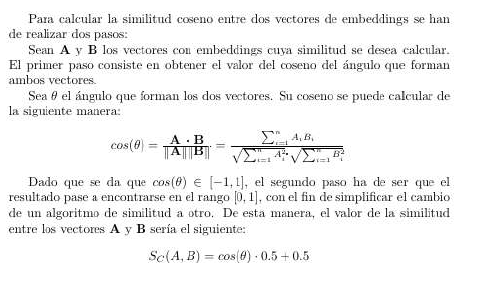
\includegraphics[width=0.8\textwidth]{Chapters/cap4.PNG}
    \label{fig:mi_imagen}
\end{figure}

\begin{figure}[htbp]
    \centering
    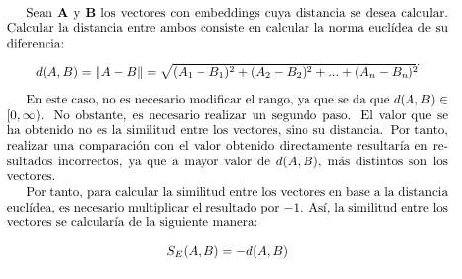
\includegraphics[width=0.8\textwidth]{Chapters/cap5.PNG}
    \label{fig:mi_imagen2}
\end{figure}

Se optó por utilizar la distancia euclídea.

\newpage

Con estas tecnologías y métodos se creó la primera versión funcional del Copilot, de la que sugieron múltiples versiones y mejoras que se aplicaron en cada una de ellas.

Algunas de las mejoras que se fueron aplicando tras prueba y error:

\begin{itemize}
    \item Se realizaron pruebas con diferentes modelos de \href{https://ollama.com/}{\bold{Ollama}} y se optó por el codellama-instruct, por su capacidad para generar código correctamente y también explicarlo. Nos dimos cuenta que aún codellama siendo un modelo especializado en código, su variante Instruct le confería la capacidad de explicar código y por ende tenía un procesamiento del lenguaje natural superior que otras versiones de codellama no disponía. Probamos convirtiendo las tablas de la BDD al lenguaje natural y tanto la comprensión del modelo como la similitud de los embeddings mejoró sustancialmente.
    \begin{figure}[htbp]
        \centering
        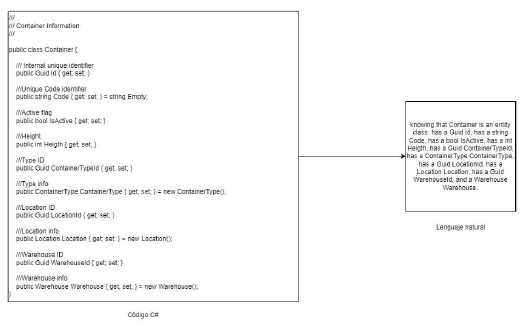
\includegraphics[width=0.9\textwidth]{Chapters/cap6.PNG}
        \label{fig:mi_imagen3}
    \end{figure}
    \item Se optó por dejar de lado \href{https://www.sqlite.org/}{\bold{SQLite}} para utilizar \href{https://www.postgresql.org/}{\bold{PostgreSQL}} junto con un módulo lllamado pgvector especializado en operaciones vectoriales que ya contaba con operaciones de distancia euclídea, por lo que no había necesidad de seguir usando código propio en \href{https://dotnet.microsoft.com/es-es/languages/csharp}{\bold{C\#}}, lo cual disminuyó enormemente los tiempos de respuesta.
    \item Se hicieron benchmarks y comparaciones entre el modo normal de funcionamiento del modelo en el que guarda el historial de todo lo que se ha escrito para poder responder a preguntas anteriores, y el modo stateless en el que no guarda información entre preguntas.
    \item Se implementó un mecanismo para detectar que la pregunta del usuario está pidiendo una explicación, preparando al modelo para que responda correctamente.
    \item Se diseñaron métodos para mejorar el tiempo de respuesta del Copilot, ya que se pretendía utilizar el hardware de los equipos de los trabajadores, por lo que tenía que ser capaz de responder en un tiempo aceptable incluso con hardware modesto.
    \item Se creó un menú inicial a la hora de arrancar el programa(se ejecuta en una terminal), en el que te permite escoger el modelo \href{https://en.wikipedia.org/wiki/Large_language_model}{\bold{LLM}} que se desee, y un submenú con todas las diferentes configuraciones creadas y tecnologías utilizadas a lo largo de las prácticas, como puede ser utilizar el Copilot en modo stateless o no, usar \href{https://www.postgresql.org/}{\bold{PostgreSQL}} o \href{https://www.sqlite.org/}{\bold{SQLite}}, o utilizar Embeddings o no. 
\end{itemize}

\subsection{Fine-tuning}

Una vez que la versión con Embeddings era funcional, y respondía en unos tiempos aceptables, se optó por probar el Fine-tuning para comparar los tiempos de respuesta.

Esta decisión era algo que personalmente desde el principio descartaba porque requiere un gasto computacional enorme y se requieren de muchísimos datos para que el Fine-tuning pueda tener un impacto significativo en el modelo, cosa en la que el tutor de prácticas estuvo de acuerdo por lo que esta etapa estaba inicialmente destinada a estimar cuanto podría llegar a costar hacerlo, y como hacerlo.

Investigando sobre el Fine-tuning descubrí un método llamado LoRA para poder hacer Fine-tuning sin tener que preentrenar el modelo \href{https://en.wikipedia.org/wiki/Large_language_model}{\bold{LLM}} entero, facilita la adaptación de modelos de lenguaje preentrenados a nuevas tareas sin un reinicio completo del entrenamiento, digamos que es como acoplar al modelo preexistente, en este caso Codellama, otro 'modelo' LoRA en tiempo de ejecución.

Esto viene muy bien a \href{https://www.mecalux.es/}{\bold{Mecalux}} no solo porque se ahorraría los costes de un Fine-tuning clásico, sino que si su base de datos crece, no es necesario volver a entrenar de cero el modelo, varios adaptadores LoRA pueden ser aplicados a un mismo modelo, y la generación de estos adaptadores es muy poco costosa computacionalmente.

Para esta nueva etapa el código en \href{https://dotnet.microsoft.com/es-es/languages/csharp}{\bold{C\#}} no cambió demasiado, y el tiempo fue destinado en como generar estos adaptadores. Llamasharp que es la biblioteca \href{https://dotnet.microsoft.com/es-es/languages/csharp}{\bold{C\#}}/.NET usada para ejecutar \href{https://en.wikipedia.org/wiki/Large_language_model}{\bold{LLM}} era incapaz de utilizar estos adaptadores correctamente, por lo que sabiendo que está basado en el proyecto original de \href{https://ollama.com/}{\bold{Ollama}} llama.cpp, escrito en \href{https://en.wikipedia.org/wiki/C_(programming_language)}{\bold{C}}/\href{https://en.wikipedia.org/wiki/C%2B%2B}{\bold{C++}} y \href{https://www.python.org/}{\bold{Python}}, se probó a utilizar los adaptadores generados en \href{https://en.wikipedia.org/wiki/C%2B%2B}{\bold{C++}} desde un Ubuntu, y se confirmó que allí si funcionaba. Aunque nos encontramos con ese bug el cual fue notificado, tuvimos la suerte de poder utilizar uno de los programas en \href{https://www.python.org/}{\bold{Python}} que vienen dentro del proyecto de llama.cpp que permite fusionar el modelo base con el adaptador LoRA y generar un modelo nuevo, que a efectos prácticos es lo mismo.

Como el proceso de generar adaptadores y combinarlos era una tarea muy tediosa y que requería de cierta complejidad y conocimientos realicé un programa en shell script para facilitar todo el proceso y de paso generar métricas. Por ejemplo la cantidad requerida de RAM para generar los adaptadores era muy elevada y sobrepasaba con creces la de los portátiles de trabajo de la empresa, por tanto el script se encarga de generar memoria swap en este caso, evitando un fallo de segmentación.

\subsection{Embeddings vs Fine-tuning}
Al finalizar las prácticas se hicieron los benchmarks pertinentes y en cuanto a tiempos de ejecución ambos eran similares, en parte porque se dedicó mucho esfuerzo en optimizar al máximo la opción embeddings, pero en la resolución de las preguntas y en coherencia tanto en las explicaciones como en la generación de código ganaba los Embeddings.

La explicación a esto además de lo previamente mencionado es que el adaptador necesita de un fichero con la información que se quiere aprender, y no había mucha información en cuanto a como de redactar dicho fichero, se probó a escribirlo en lenguaje natural y después siguiendo directrices que se usaron para entrenar a codellama, pero no se hicieron unas pruebas exhaustivas por no disponer de más tiempo.

Es probable que afinando la manera de elaborar ese fichero las comparativas cambien a favor del Fine-tuning usando LoRA.
\subsection{Esquema general del proyecto}

\begin{figure}[htbp]
    \centering
    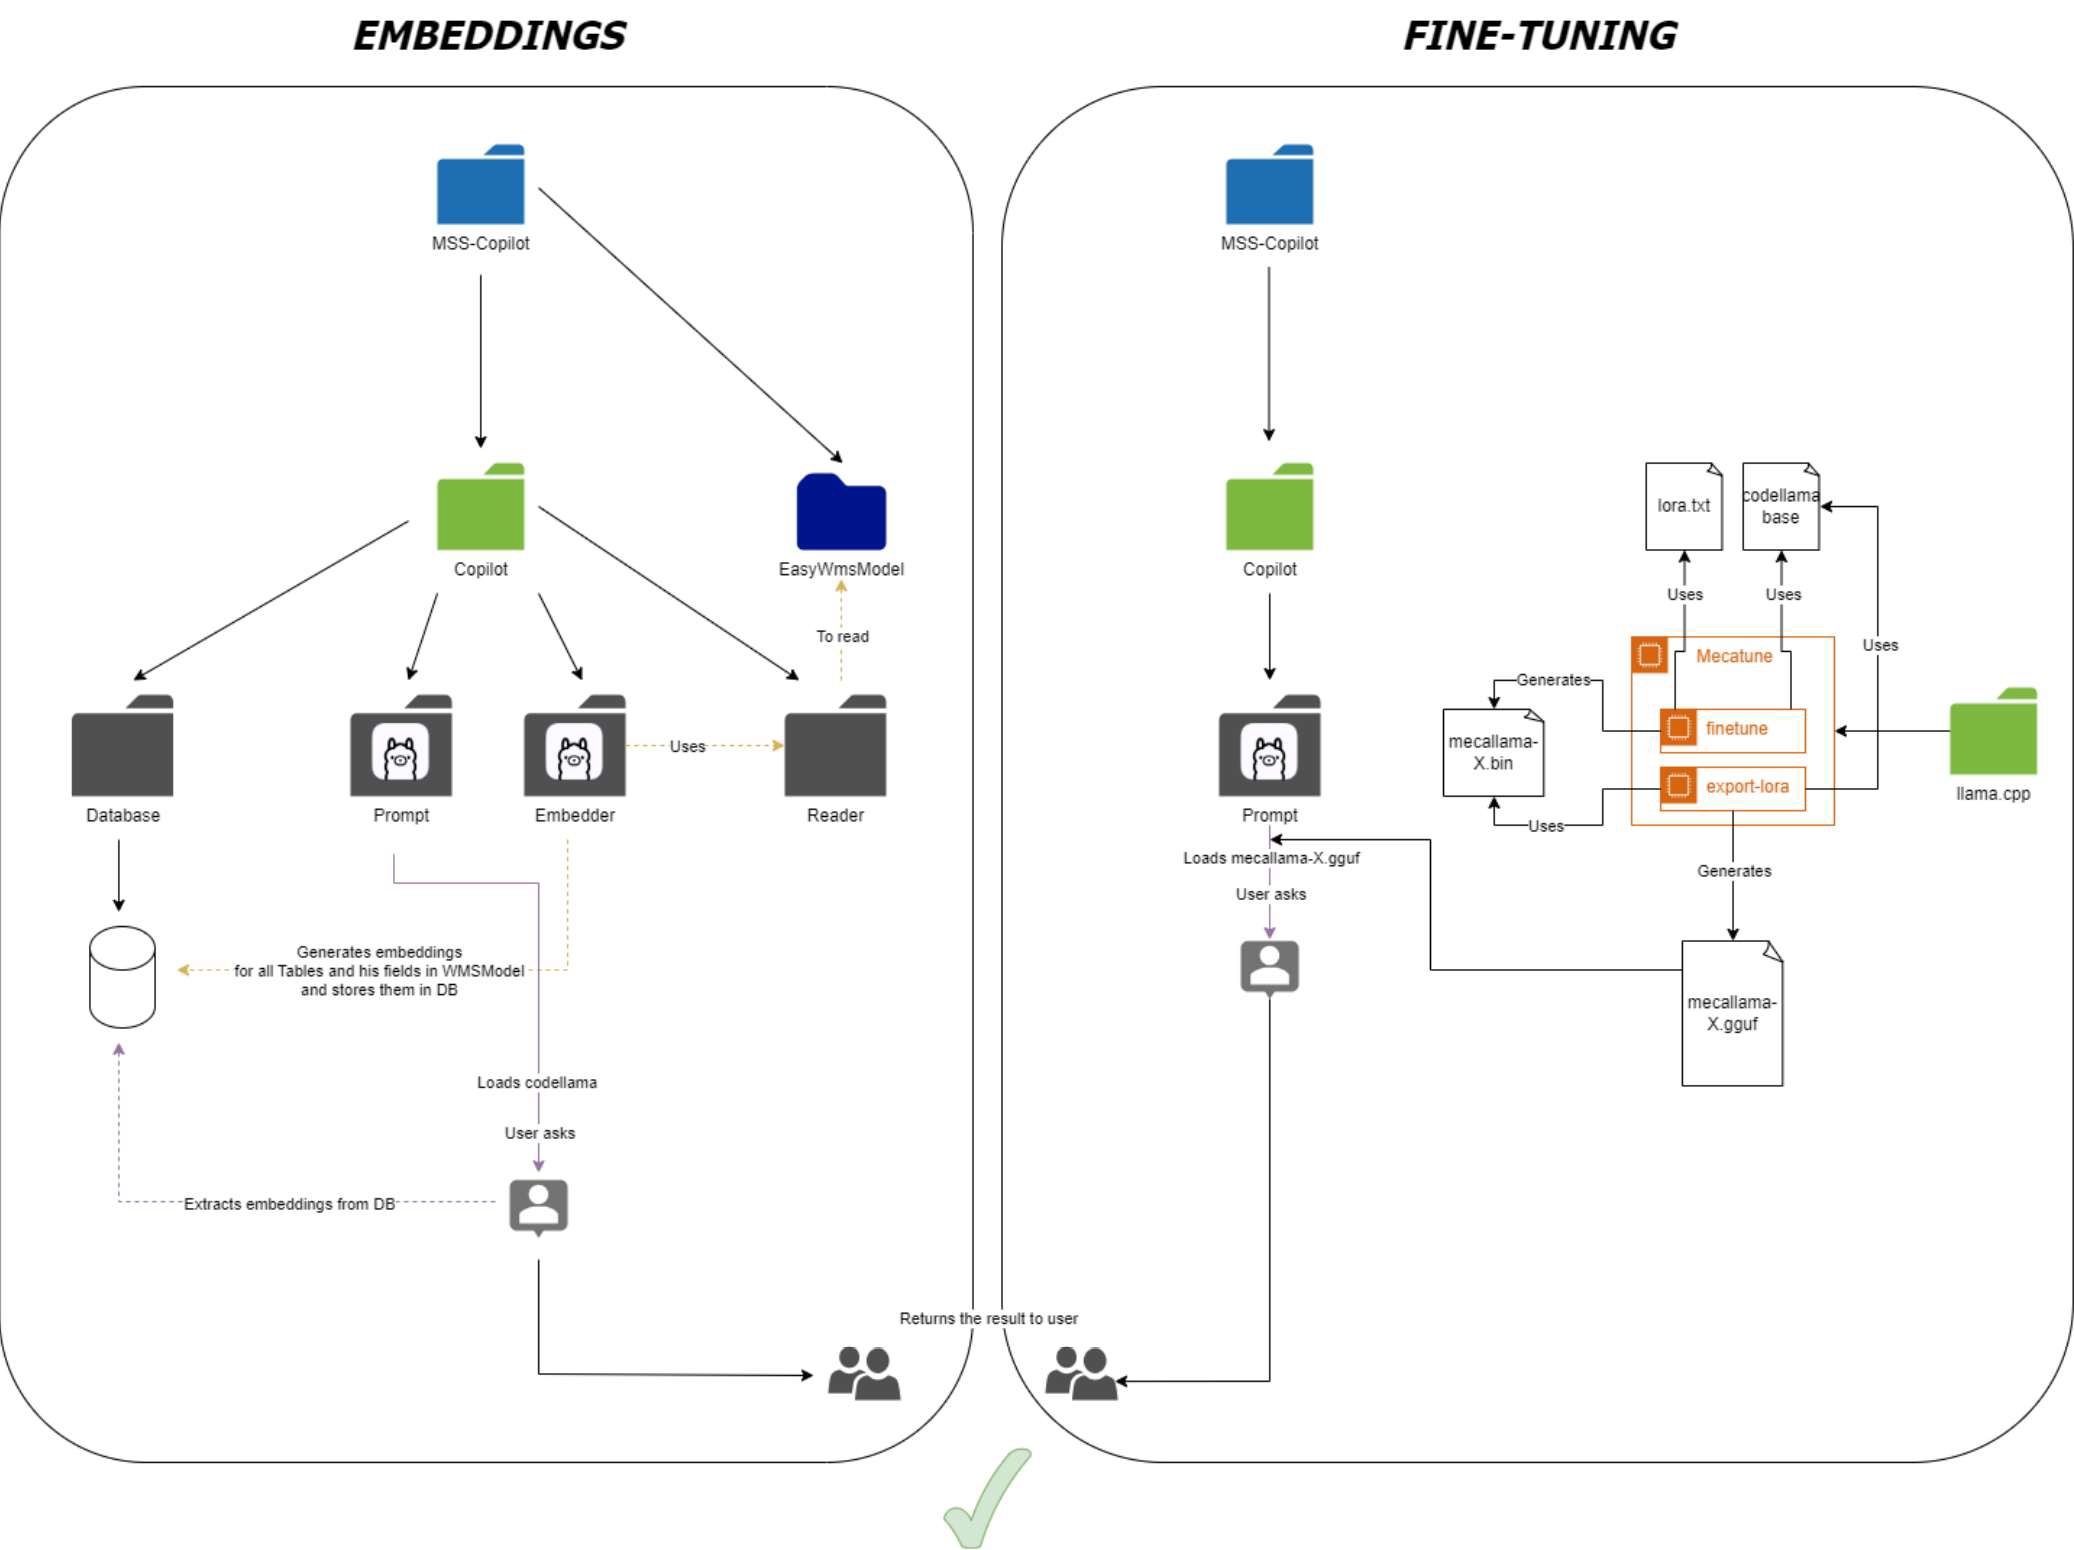
\includegraphics[width=1\textwidth]{Chapters/image.PNG}
    \label{fig:mi_imagen4}
\end{figure}

\newpage

\section{Relación de las tareas desarrolladas
con los conocimientos adquiridos
en los estudios universitarios}
Al reflexionar sobre mis estudios, identifico varias asignaturas y temas que han sido particularmente relevantes y valiosos para mi formación. Estos incluyen:
\begin{itemize}
    \item \bold{Sistemas Inteligentes e Inteligencia de Negocio:} Cursé Sistemas Inteligentes en el 2020-2021 e Inteligencia de Negocio el año posterior, así que no puedo ser muy específico en cuanto al temario dado pero creo que son dos asignaturas que aunque hayan pasado 2-3 años desde que las he cursado me han permitido realizar las prácticas con un contexto general sobre la inteligencia artificial, conceptos como el procesamiento del lenguaje natural, o el entendimiento de como funciona un \href{https://en.wikipedia.org/wiki/Large_language_model}{\bold{LLM}} por debajo, y conceptos como tokens, training data, sobreajuste, subajuste, etc..
    \item \bold{Bases de Datos y Sistemas de Información:}  Bases de datos ha sido una asignatura esencial ya no solo por el hecho de almacenar la información de los Embeddings sino que en el contexto del programa, que es un asistente de sentencias SQL, ha sido esencial para poder probar luego la IA y saber que las queries que me daba eran correctas o no, además de que en esta asignatura aprendí \href{https://www.postgresql.org/}{\bold{PostgreSQL}}. Destaco también la asignatura de Sistemas de Información porque en ella utilicé \href{https://www.sqlite.org/}{\bold{SQLite}}, y fue la primera toma de contacto que tuve entre backend y BDD.
    \item \bold{Metodología de la Programación y Tecnologías y Paradigmas de la Programación:} Del caso de Metodología de la Programación recalcar la importancia de haber aprendido polimorfismo, y de Paradigmas de la Programación los patrones de diseño, cabe recalcar que prácticamente todo el conocimiento backend de la carrera ha sido en \href{https://www.java.com/en/}{\bold{Java}}, y que \href{https://dotnet.microsoft.com/es-es/languages/csharp}{\bold{C\#}} se utiliza únicamente en las prácticas de Seguridad y muy muy superficialmente, pero con los conocimientos de estas asignaturas no ha sido nada complicado hacer una abstracción de todos estos conocimientos de programación y aplicarlos en \href{https://dotnet.microsoft.com/es-es/languages/csharp}{\bold{C\#}}, la adaptación fue bastante más amena de la que pensaba en un principio. 
    \item \bold{Programación Concurrente y Paralela:} Si bien he utilizado paralelización de tareas ha sido de una manera muy básica, ya que las librerías se encargaban de hacerlo todo más fácil, pero los conocimientos teóricos han sido útiles de igual manera, y recalcar sobre todo los contenidos aprendidos respecto a 
    \href{https://es.wikipedia.org/wiki/CUDA}{\bold{CUDA}}, el modelo \href{https://en.wikipedia.org/wiki/Large_language_model}{\bold{LLM}} se puede ejecutar tanto en CPU como GPU, y toda la problemática que implica programar utilizando 
    \href{https://es.wikipedia.org/wiki/CUDA}{\bold{CUDA}} se me hizo muy amena gracias a esta asignatura, sin ella se me hubiese hecho muy cuesta arriba este aspecto.
    \newpage
    \item \bold{Configuración y Evaluación de Sistemas:} Me ha parecido una asignatura fundamental y que he recordado muchas veces a la hora de realizar las prácticas, he tenido que hacer muchísimos benchmarks y pruebas de rendimiento frente a muchas casuísticas y hacer muchas gráficas que gracias a esta asignatura considero que he hecho correctamente. Me gustaría comentar que gracias al paradigma de esta asignatura me percaté que el programa daba unos tiempos de respuesta anormales y que eran debidos a dos factores principales, uno que la capacidad de cómputo era tal que el procesador llegaba al estrangulamiento térmico y capaba sus capacidades para no prenderse fuego, y que la discrepancia entre múltiples equipos del departamento se debía a que muchos de estos eran portátiles y su potencia se veía enormemente reducida cuando no estaban enchufados a la corriente independientemente de que se hubiese configurado Windows para que esto no pasase.
    \item \bold{Sistemas Distribuidos y Algoritmia:} Son dos asignaturas que en lo que es conocimientos no me han servido especialmente, quizás si Algoritmia de manera más subconsciente, pero son asignaturas en las que utilicé muchísimo \href{https://en.wikipedia.org/wiki/C_(programming_language)}{\bold{C}} y \href{https://en.wikipedia.org/wiki/C%2B%2B}{\bold{C++}}, lo cual me vino bien de cara a la parte de Fine-tuning.
    \item \bold{Sistemas Operativos:} Considero que es otra de las asignaturas fundamentales, ya que nos enseñan a manejarnos bien en un sistema basado en Linux, crear shell-scripts, y hacernos descubrir este aspecto de la informática y la importancia de la consola, que de no ser por esta asignatura, probablemente no tendría los conocimientos que tengo hoy en día. 
\end{itemize}

% Chapter 3
\chapter{Lecciones aprendidas y conclusiones}
Durante el desarrollo de mis prácticas, he adquirido y puesto en prueba tanto habilidades blandas como habilidades técnicas, alineadas con las competencias básicas, generales, y específicas de mi grado en Ingeniería Informática en Tecnologías de la Información.

Nunca había utilizado \href{https://dotnet.microsoft.com/es-es/languages/csharp}{\bold{C\#}}, pero confiaba en la capacidad de abstraer mis conocimientos de otros lenguajes POO, y considero que no tengo nociones muy avanzadas en cuanto a inteligencia artificial respecta, pero si interés por la temática, ya que tenía pensado realizar por mi cuenta algo bastante parecido a lo que se requería en la oferta, por lo que me aventuré a hacerme cargo de las responsabilidades que se requerían para las prácticas, y estoy muy contento con la decisión.

He aprendido muchísimo más del campo de la inteligencia artificial, y he disfrutado mucho de toda la labor de investigación que realizamos para poder ofrecer soluciones al proyecto, conceptos como LoRA, RAG, o el descubrimiento de modelos \href{https://en.wikipedia.org/wiki/Large_language_model}{\bold{LLM}} emergentes que usan 2 bits para los pesos permitiendo ejecutar estos modelos en dispositivos de recursos limitados como podrían ser dispositivos móviles, entre otros muchos más conocimientos adquiridos.

He experimentado una gran satisfacción durante mis prácticas, ya que he tenido la oportunidad de trabajar con una variedad de herramientas, tecnologías y librerías (pgAdmin, \href{https://www.sqlite.org/}{\bold{SQLite}}, 
\href{https://es.wikipedia.org/wiki/CUDA}{\bold{CUDA}}, pgvector, llamasharp, llama.cpp), así como con diferentes lenguajes de programación (\href{https://en.wikipedia.org/wiki/C_(programming_language)}{\bold{C}}, \href{https://en.wikipedia.org/wiki/C%2B%2B}{\bold{C++}}, \href{https://dotnet.microsoft.com/es-es/languages/csharp}{\bold{C\#}}, \href{https://www.python.org/}{\bold{Python}}, Shell, PL/pgSQL) y sistemas operativos (Windows, WSL). Esta diversidad ha sido muy gratificante y ha complementado mi deseo de adquirir un conocimiento amplio y una visión general de múltiples áreas.

Los problemas que tuve con la librería de llamasharp me hizo crear mis primeras issues en GitHub lo cual junto a el uso de Git para el proyecto de MSSCopilot me acercó más a los conocimientos necesarios y buenas prácticas para el desarrollo de código colaborativo. 
\newpage
La necesidad de comunicarme con mi compañero de prácticas de manera efectiva y aprovechar al máximo las virtudes de cada uno siendo consciente de nuestras flaquezas y diferencias me ha servido mucho como crecimiento personal a la hora de trabajar en equipo, un poco de liderazgo, y sobre todo de adaptabilidad y resolución de problemas.

En general ha sido una experiencia en la que aunque la tutela del tutor ha sido excelente y ha estado presente y preocupado por nosotros en todo momento a pesar de sus responsabilidades, ha habido bastante autonomía y he sentido que se le ha dado mucha importancia a la capacidad de resolución de problemas y el pensamiento crítico lo cual valoro muchísimo.

Todo el departamento de Data Analytics me trató excelentemente y he tenido un trato muy cercano, en general con todo el personal de la empresa pero especialmente con ellos. Ha sido muy enriquecedor en todos los sentidos ver como opera una empresa de tal importancia como es \href{https://www.mecalux.es/}{\bold{Mecalux}}. 

\section{Análisis de las características y perfil profesional del puesto desempeñado}

Durante mis prácticas en la empresa Mecalux, desempeñé el rol de desarrollador de software, con un enfoque particular en la inteligencia artificial y el desarrollo de aplicaciones. Estas se han alineado perfectamente con mi perfil profesional como futuro egresado de Ingeniería Informática, poniendo a prueba y desarrollando competencias que considero esenciales para mi carrera. Desde el inicio, se esperaba de mí un ojo crítico y habilidades avanzadas para resolver problemas, así como buenas habilidades de comunicación y pensamiento crítico, todas características indispensables para un ingeniero informático. A lo largo de mi formación y durante estas prácticas, he tenido la oportunidad de aplicar muchas de las competencias clave que se esperan de nosotros al finalizar el grado. 

A continuación, se presenta un análisis detallado de las características y el perfil profesional del puesto que desempeñé:

\subsection{Descripción del puesto}
El rol principal involucró el desarrollo de soluciones de inteligencia artificial utilizando diversas herramientas y tecnologías. Las responsabilidades específicas incluyeron la programación en lenguajes como \href{https://dotnet.microsoft.com/es-es/languages/csharp}{\bold{C\#}}, \href{https://www.python.org/}{\bold{Python}}, Shell, \href{https://en.wikipedia.org/wiki/C_(programming_language)}{\bold{C}} y \href{https://en.wikipedia.org/wiki/C%2B%2B}{\bold{C++}}, el uso de bases de datos como \href{https://www.sqlite.org/}{\bold{SQLite}} y \href{https://www.postgresql.org/}{\bold{PostgreSQL}}, y la implementación de algoritmos de inteligencia artificial.
\newpage
\subsection{Habilidades y competencias requeridas}
El puesto requirió una sólida comprensión de los principios de programación orientada a objetos, habilidades en el manejo de bases de datos, y conocimientos básicos en inteligencia artificial. Además, se necesitaba la capacidad de resolver problemas técnicos complejos y de trabajar de manera colaborativa en un equipo con cierta autonomía.

\subsection{Formación y conocimientos}
Mi formación en la carrera proporcionó una base sólida en programación y sistemas operativos, que fue crucial para cumplir con las responsabilidades del puesto. 

Sin embargo, la necesidad de aprender y adaptarme a nuevas tecnologías como \href{https://dotnet.microsoft.com/es-es/languages/csharp}{\bold{C\#}} y herramientas específicas de inteligencia artificial destacó la importancia de la capacidad de aprendizaje autónomo.

\subsection{Desarrollo profesional}
Estas prácticas me permitieron adquirir nuevas habilidades técnicas, como el uso de librerías de IA emergentes y una mejora sustancial en la gestión de proyectos de software colaborativo mediante Git. También mejoré mis competencias blandas, especialmente en comunicación efectiva y trabajo en equipo.

\subsection{Alineación con el perfil profesional}
El puesto se alinea estrechamente con mis objetivos profesionales de trabajar en el desarrollo de software y aplicaciones de inteligencia artificial. La experiencia práctica adquirida complementa mi formación académica y fortalece mi perfil profesional como futuro ingeniero informático.

\subsection{Evaluación personal}
Durante las prácticas, pude aplicar muchas de las competencias adquiridas en mi formación, tales como la capacidad de resolver problemas (GTR1), actuar autónomamente (GTR3), y comunicarme efectivamente (GTR6). Identifiqué áreas de mejora en el manejo avanzado de ciertas tecnologías y en la profundización de conocimientos en inteligencia artificial, que son objetivos para mi desarrollo futuro.

En resumen, las prácticas no solo me permitieron aplicar y expandir mis conocimientos técnicos, sino que también fueron fundamentales para mi crecimiento profesional y personal, alineándose perfectamente con los de la carrera.

\section{Sugerencias}
Aunque me gustaría ofrecer sugerencias constructivas para mejorar el proceso de prácticas, debo admitir que las experiencias vividas han sido increíblemente satisfactorias y considero que se han abordado de manera casi perfecta. Sin embargo, siempre hay aspectos que pueden ser optimizados para futuros alumnos.

Durante las prácticas, la comunicación se llevó a cabo principalmente a través de Teams, una plataforma que, si bien resultó familiar y eficiente debido a su uso constante durante mi formación académica, eché de menos la utilización de software especializado para empresas, como Jira o Slack. Estas herramientas, utilizadas por otros compañeros en sus prácticas, ofrecen funcionalidades específicas que podrían haber mejorado aún más la gestión y coordinación del proyecto. No obstante, entiendo que la elección de Teams se haya debido a su integración con la cuenta de Microsoft proporcionada al inicio de las prácticas, lo cual facilita la gestión de usuarios y recursos.

En cuanto a la experiencia personal, he notado que en algunas empresas, los alumnos reciben merchandising como mochilas, camisetas o termos. Esta práctica no solo contribuye a la promoción de la empresa, sino que también motiva a los alumnos al sentirse parte de la organización. Considero que proporcionar este tipo de obsequios podría fortalecer aún más el vínculo entre los estudiantes y Mecalux Software Solutions, y ayudar a difundir su nombre dentro del círculo académico de informática, lo cual sería beneficioso para ambas partes.

%----------------------------------------------------------------------------------------
%	THESIS CONTENT - APPENDICES
%----------------------------------------------------------------------------------------

\appendix % Cue to tell LaTeX that the following "chapters" are Appendices

% Include the appendices of the thesis as separate files from the Appendices folder
% Uncomment the lines as you write the Appendices

%\include{Appendices/AppendixA}

%----------------------------------------------------------------------------------------
%	BIBLIOGRAPHY
%----------------------------------------------------------------------------------------

%\printbibliography[heading=bibintoc]
%\printbibliography

%----------------------------------------------------------------------------------------

\end{document}  
